\documentclass[oneside,openany,headings=optiontotoc,11pt,numbers=noenddot]{scrreprt}

\usepackage[a4paper]{geometry}
\usepackage[utf8]{inputenc}
\usepackage[T1]{fontenc}
\usepackage{lmodern}
\usepackage[ngerman]{babel}
\usepackage{ngerman}

\usepackage[onehalfspacing]{setspace}

\usepackage{fancyhdr}
\usepackage{fancybox}

\usepackage{rotating}
\usepackage{varwidth}

%Struktogramme
\usepackage[german,curves]{struktex}

\usepackage{pdflscape}
\usepackage{changepage}
\usepackage{graphicx}
\usepackage[bottom]{footmisc}
\usepackage{transparent}
\usepackage{graphbox}
\graphicspath{
	{Pics/PDFs/}
	{Pics/JPGs/}
	{Pics/PNGs/}
}
\usepackage{caption}
\usepackage{wrapfig}
\usepackage{marginnote}
\usepackage{tabularx}
\usepackage{dashrule}
\usepackage{soulutf8}
\usepackage{hhline}
%arydshln suppresses vertical lines in table
%\usepackage{arydshln}
\usepackage{multirow}
\usepackage{enumerate}
\usepackage[hidelinks]{hyperref}
\usepackage{listings}

\usepackage[table]{xcolor}
\usepackage{array}
\usepackage{enumitem,amssymb,amsmath}
\usepackage{interval}
\usepackage{cancel}
\usepackage{stmaryrd}
\usepackage{wasysym}
\usepackage{polynom}
\usepackage{diagbox}
\usepackage{dashrule}
\usepackage{framed}
\usepackage{mdframed}
\usepackage{karnaugh-map}
\usepackage{pdfpages}

\usepackage{blindtext}

\usepackage{eso-pic}

\usepackage{amssymb}
\usepackage{eurosym}

\usepackage[pages=some]{background}
\pagestyle{headings}
\renewcommand{\headrulewidth}{0.2pt}
\renewcommand{\footrulewidth}{0.2pt}
\newcommand*{\underdownarrow}[2]{\ensuremath{\underset{\overset{\Big\downarrow}{#2}}{#1}}}
\setlength{\fboxsep}{5pt}
\newcommand{\explainBelow}[3]{\underbrace{#1}_{\parbox{\widthof{#3}}{\footnotesize\raggedright #2}}}
\newcommand{\explainAbove}[3]{\overbrace{#1}^{\parbox{\widthof{#3}}{\footnotesize\raggedright #2}}}
\newcommand\footnoteref[1]{\protected@xdef\@thefnmark{\ref{#1}}\@footnotemark}


% Codestyle defined
\definecolor{codegreen}{rgb}{0,0.6,0}
\definecolor{codegray}{rgb}{0.5,0.5,0.5}
\definecolor{codepurple}{rgb}{0.58,0,0.82}
\definecolor{backcolour}{rgb}{0.95,0.95,0.92}
\definecolor{deepgreen}{rgb}{0,0.5,0}
\definecolor{darkblue}{rgb}{0,0,0.65}
\definecolor{mauve}{rgb}{0.40, 0.19,0.28}
\colorlet{exceptioncolour}{yellow!50!red}
\colorlet{commandcolour}{blue!60!black}
\colorlet{numpycolour}{blue!60!green}
\colorlet{specmethodcolour}{violet}

%Neue Spaltendefinition
\newcolumntype{L}[1]{>{\raggedright\let\newline\\\arraybackslash\hspace{0pt}}m{#1}}
\newcolumntype{M}{>{\centering\arraybackslash}X}
\newcommand{\cmnt}[1]{\ignorespaces}
%Textausrichtung ändern
\newcommand\tabrotate[1]{\rotatebox{90}{\raggedright#1\hspace{\tabcolsep}}}

%Intervall-Konfig
\intervalconfig {
	soft open fences
}

%Bash
\lstdefinestyle{BashInputStyle}{
	language=bash,
	basicstyle=\small\sffamily,
	backgroundcolor=\color{backcolour},
	columns=fullflexible,
	backgroundcolor=\color{backcolour},
	breaklines=true,
}
%Java
\lstdefinestyle{JavaInputStyle}{
	language=Java,
	backgroundcolor=\color{backcolour},
	aboveskip=1mm,
	belowskip=1mm,
	showstringspaces=false,
	columns=flexible,
	basicstyle={\footnotesize\ttfamily},
	numberstyle={\tiny},
	numbers=none,
	keywordstyle=\color{purple},,
	commentstyle=\color{deepgreen},
	stringstyle=\color{blue},
	emph={out},
	emphstyle=\color{darkblue},
	emph={[2]rand},
	emphstyle=[2]\color{specmethodcolour},
	breaklines=true,
	breakatwhitespace=true,
	tabsize=2,
}
%Python
\lstdefinestyle{PythonInputStyle}{
	language=Python,
	alsoletter={1234567890},
	aboveskip=1ex,
	basicstyle=\footnotesize,
	breaklines=true,
	breakatwhitespace= true,
	backgroundcolor=\color{backcolour},
	commentstyle=\color{red},
	otherkeywords={\ , \}, \{, \&,\|},
	emph={and,break,class,continue,def,yield,del,elif,else,%
		except,exec,finally,for,from,global,if,import,in,%
		lambda,not,or,pass,print,raise,return,try,while,assert},
	emphstyle=\color{exceptioncolour},
	emph={[2]True,False,None,min},
	emphstyle=[2]\color{specmethodcolour},
	emph={[3]object,type,isinstance,copy,deepcopy,zip,enumerate,reversed,list,len,dict,tuple,xrange,append,execfile,real,imag,reduce,str,repr},
	emphstyle=[3]\color{commandcolour},
	emph={[4]ode, fsolve, sqrt, exp, sin, cos, arccos, pi,  array, norm, solve, dot, arange, , isscalar, max, sum, flatten, shape, reshape, find, any, all, abs, plot, linspace, legend, quad, polyval,polyfit, hstack, concatenate,vstack,column_stack,empty,zeros,ones,rand,vander,grid,pcolor,eig,eigs,eigvals,svd,qr,tan,det,logspace,roll,mean,cumsum,cumprod,diff,vectorize,lstsq,cla,eye,xlabel,ylabel,squeeze},
	emphstyle=[4]\color{numpycolour},
	emph={[5]__init__,__add__,__mul__,__div__,__sub__,__call__,__getitem__,__setitem__,__eq__,__ne__,__nonzero__,__rmul__,__radd__,__repr__,__str__,__get__,__truediv__,__pow__,__name__,__future__,__all__},
	emphstyle=[5]\color{specmethodcolour},
	emph={[6]assert,range,yield},
	emphstyle=[6]\color{specmethodcolour}\bfseries,
	emph={[7]Exception,NameError,IndexError,SyntaxError,TypeError,ValueError,OverflowError,ZeroDivisionError,KeyboardInterrupt},
	emphstyle=[7]\color{specmethodcolour}\bfseries,
	emph={[8]taster,send,sendMail,capture,check,noMsg,go,move,switch,humTem,ventilate,buzz},
	emphstyle=[8]\color{blue},
	keywordstyle=\color{blue}\bfseries,
	rulecolor=\color{black!40},
	showstringspaces=false,
	stringstyle=\color{deepgreen}
}

\lstset{literate=%
	{Ö}{{\"O}}1
	{Ä}{{\"A}}1
	{Ü}{{\"U}}1
	{ß}{{\ss}}1
	{ü}{{\"u}}1
	{ä}{{\"a}}1
	{ö}{{\"o}}1
}

% Neue Klassenarbeits-Umgebung
\newenvironment{worksheet}[3]
% Begin-Bereich
{
	\newpage
	\sffamily
	\setcounter{page}{1}
	\ClearShipoutPicture
	\AddToShipoutPicture{
		\put(55,761){{
				\mbox{\parbox{385\unitlength}{\tiny \color{codegray}BBS I Mainz, #1 \newline #2
						\newline #3
					}
				}
			}
		}
		\put(455,761){{
				\mbox{\hspace{0.3cm}
\includegraphics[width=0.2\textwidth]{../../logo.pdf}}
			}
		}
	}
}
% End-Bereich
{
	\clearpage
	\ClearShipoutPicture
}

\geometry{left=2.50cm,right=2.50cm,top=2.00cm,bottom=1.00cm,includeheadfoot}

\begin{document}
	\begin{worksheet}{HBF IT 17A}{Grundstufe}{Vorbereitung Klassenarbeit}
		\begin{framed}
			\noindent\normalsize
			\textbf{Aufgabe 1}\\
			Beantworten Sie die nachfolgenden Fragen.
			\paragraph{(a)} Wie bestimmen Sie die Nullstelle einer linearen Funktion?
			\paragraph{(b)} Welche Möglichkeiten gibt es, die Nullstellen einer quadratischen Funktion zu bestimmen?
			\paragraph{(c)} Gegeben ist eine Funktion dritten Grades. Wie gehen Sie vor, um die Nullstellen dieser Funktion zu bestimmen?
			\paragraph{(d)} Um die Nullstellen einer Funktion vom Grad 4 zu berechnen, gehen Sie wie vor?\\
			\hdashrule[0.5ex][x]{\textwidth}{0.1mm}{8mm 2pt}\\
			\textbf{Aufgabe  2}\\
			\par
			\textbf{Aufgabe 2.1}\\
			Gegeben sind die folgenden Funktionen. Bestimmen Sie die Nullstellen.\\
			\begin{align*}
				&(a)\ f(x) = 5x + 10\\
				&(b)\ f(x) = x^2 - 15x\\
				&(c)\ f(x) = \frac{1}{4}x^2 -25\\
				&(d)\ f(x) = 4x^2 +12x\\
				&(e)\ f(x) = -3x^2 +15x -18\\
				&(f)\ f(x) = -x^3+2x^2-\frac{1}{2}\\
				&(g)\ f(x) = -0.8x^4 - 2x^3 + 5x^2\\
				&(h)\ f(x) = x^4 -4x^2 +3\\
				&(i)\ f(x) = x^3-4x^2 +3x\\
				&(j)\ f(x) = -5x^3 +25x^2-20
			\end{align*}\\
			\hdashrule[0.2ex][x]{\textwidth}{0.2mm}{1mm 3pt}\\
			\indent\textbf{Aufgabe 2.2}\\
			Geben Sie jeweils das Verfahren an, welches Sie verwendet haben und begründen Sie, ob dieses das sinnvollste ist.\\
			\hdashrule[0.5ex][x]{\textwidth}{0.1mm}{8mm 2pt}\\
			\textbf{Aufgabe 3}\\
			Geben Sie die erste (\(f'(x)\)) und zweite (\(f''(x)\)) Ableitung der Funktionen aus Aufgabenteil \textit{2.1} an.\\
			\textbf{Aufgabe 4}\\
			\par\noindent
			Markieren Sie die markanten Stellen in den nachfolgenden Funktionsgraphen.\\
			Beschriften Sie die Stellen entsprechend (\(N, HOP, TIP, WP_{LR}, WP_{RL}\)).\\
			\par
			\begin{tabularx}{\textwidth}{X|X}
				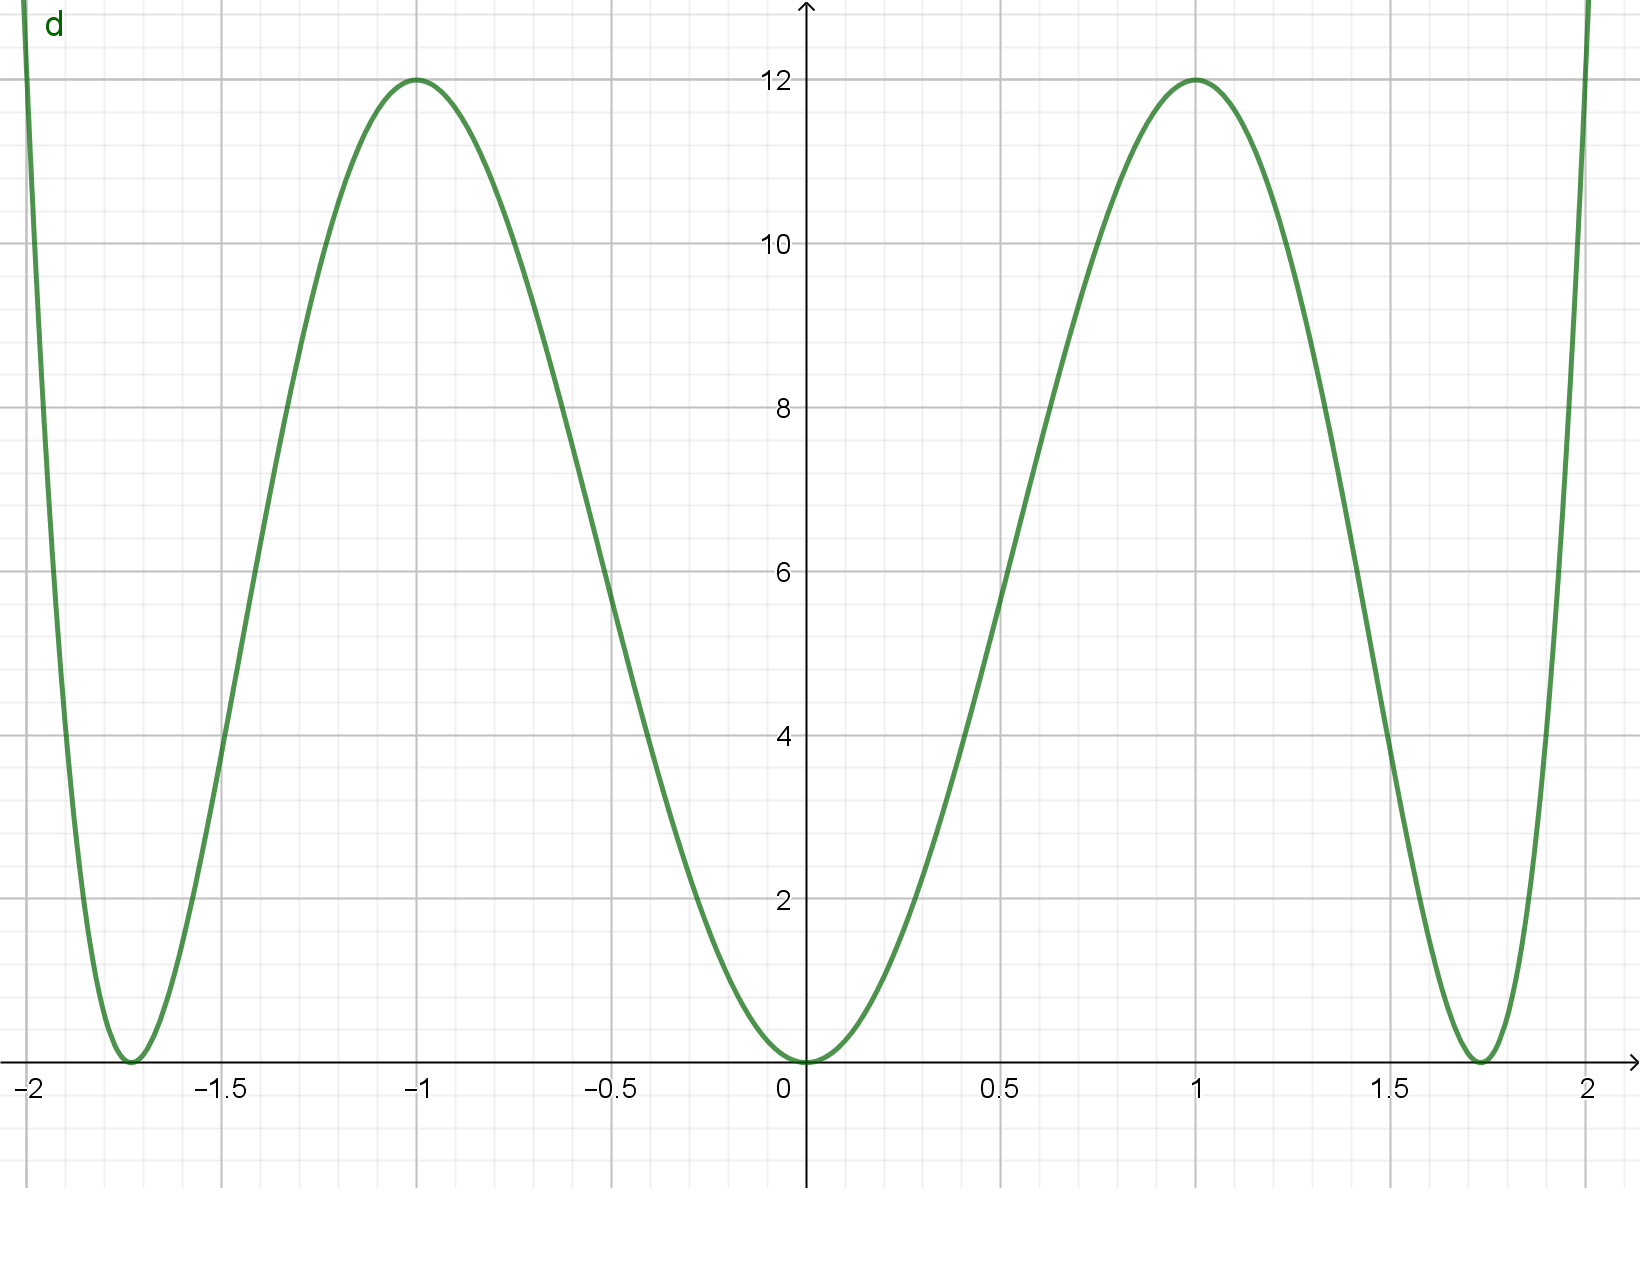
\includegraphics[scale=0.25]{Bilder/KAUebungBilder/d0.png} & 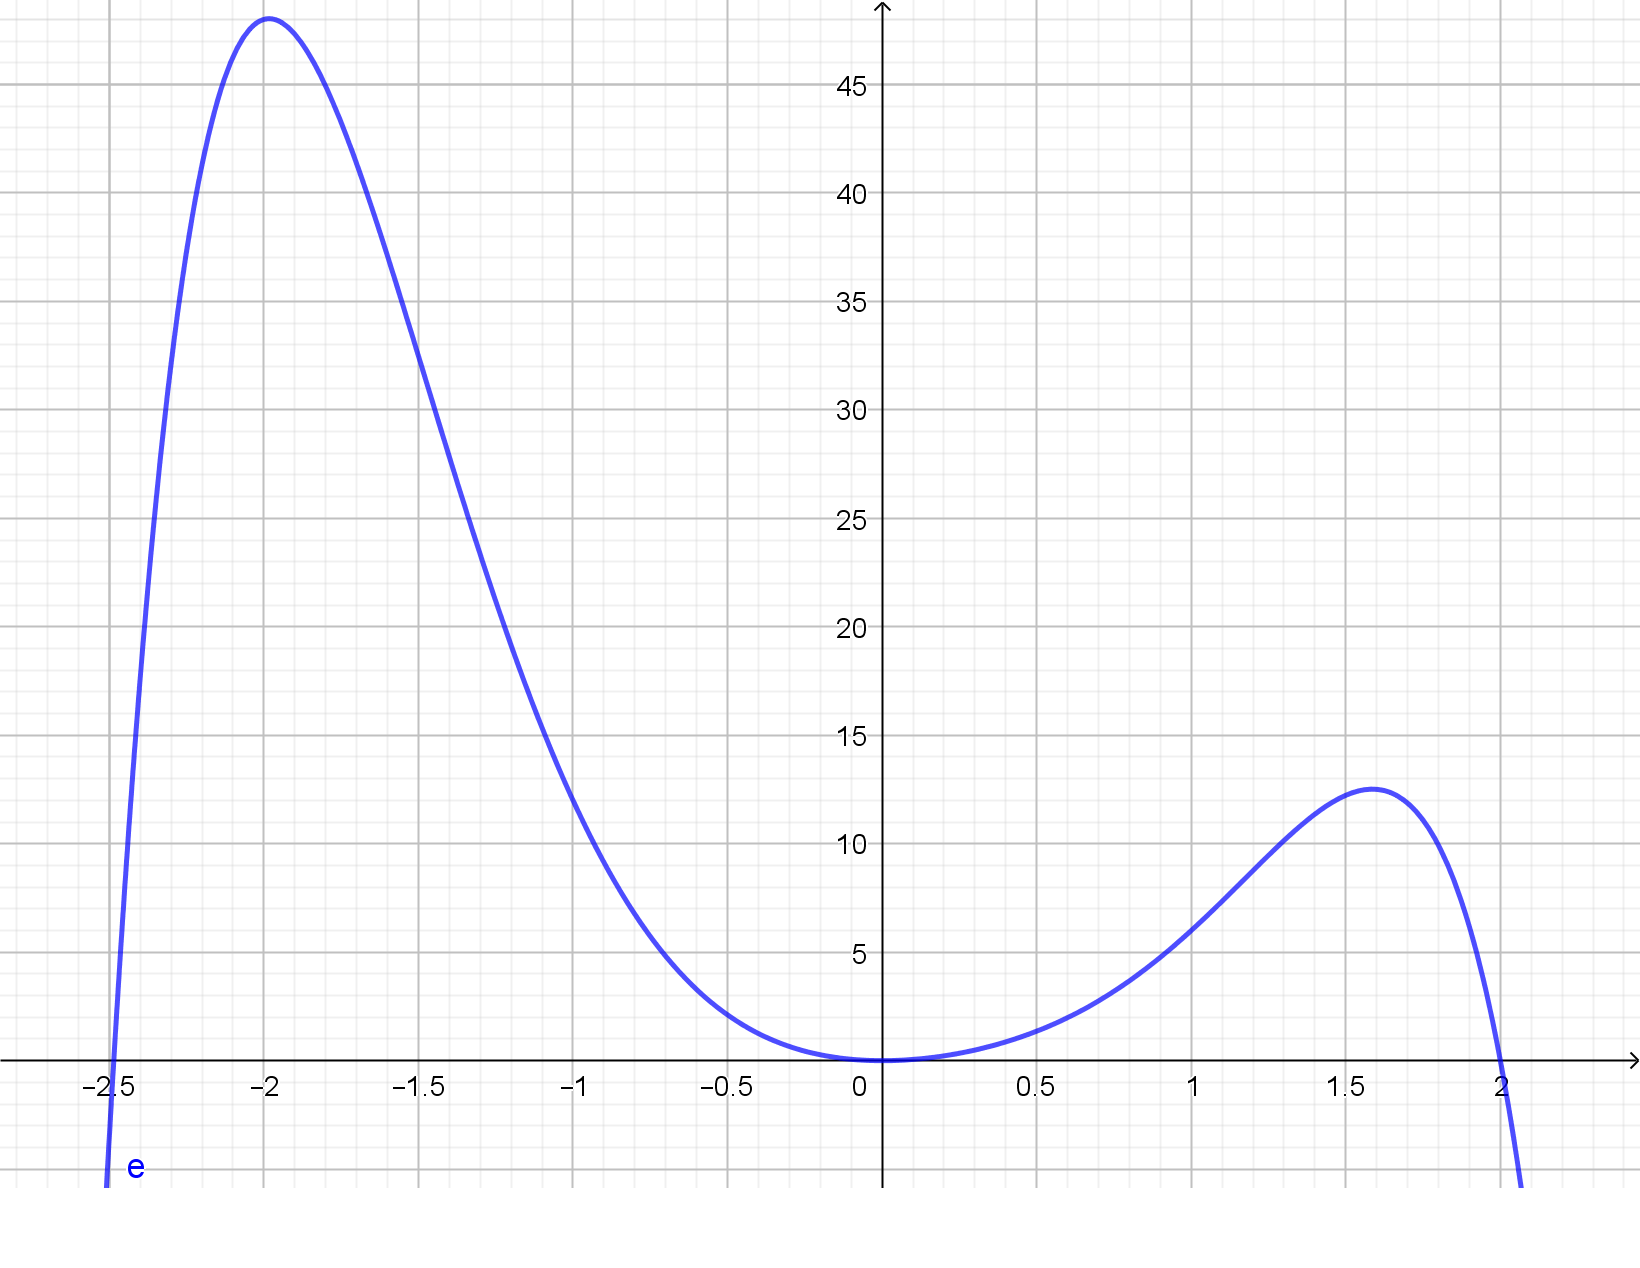
\includegraphics[scale=0.25]{Bilder/KAUebungBilder/e0.png} \\
				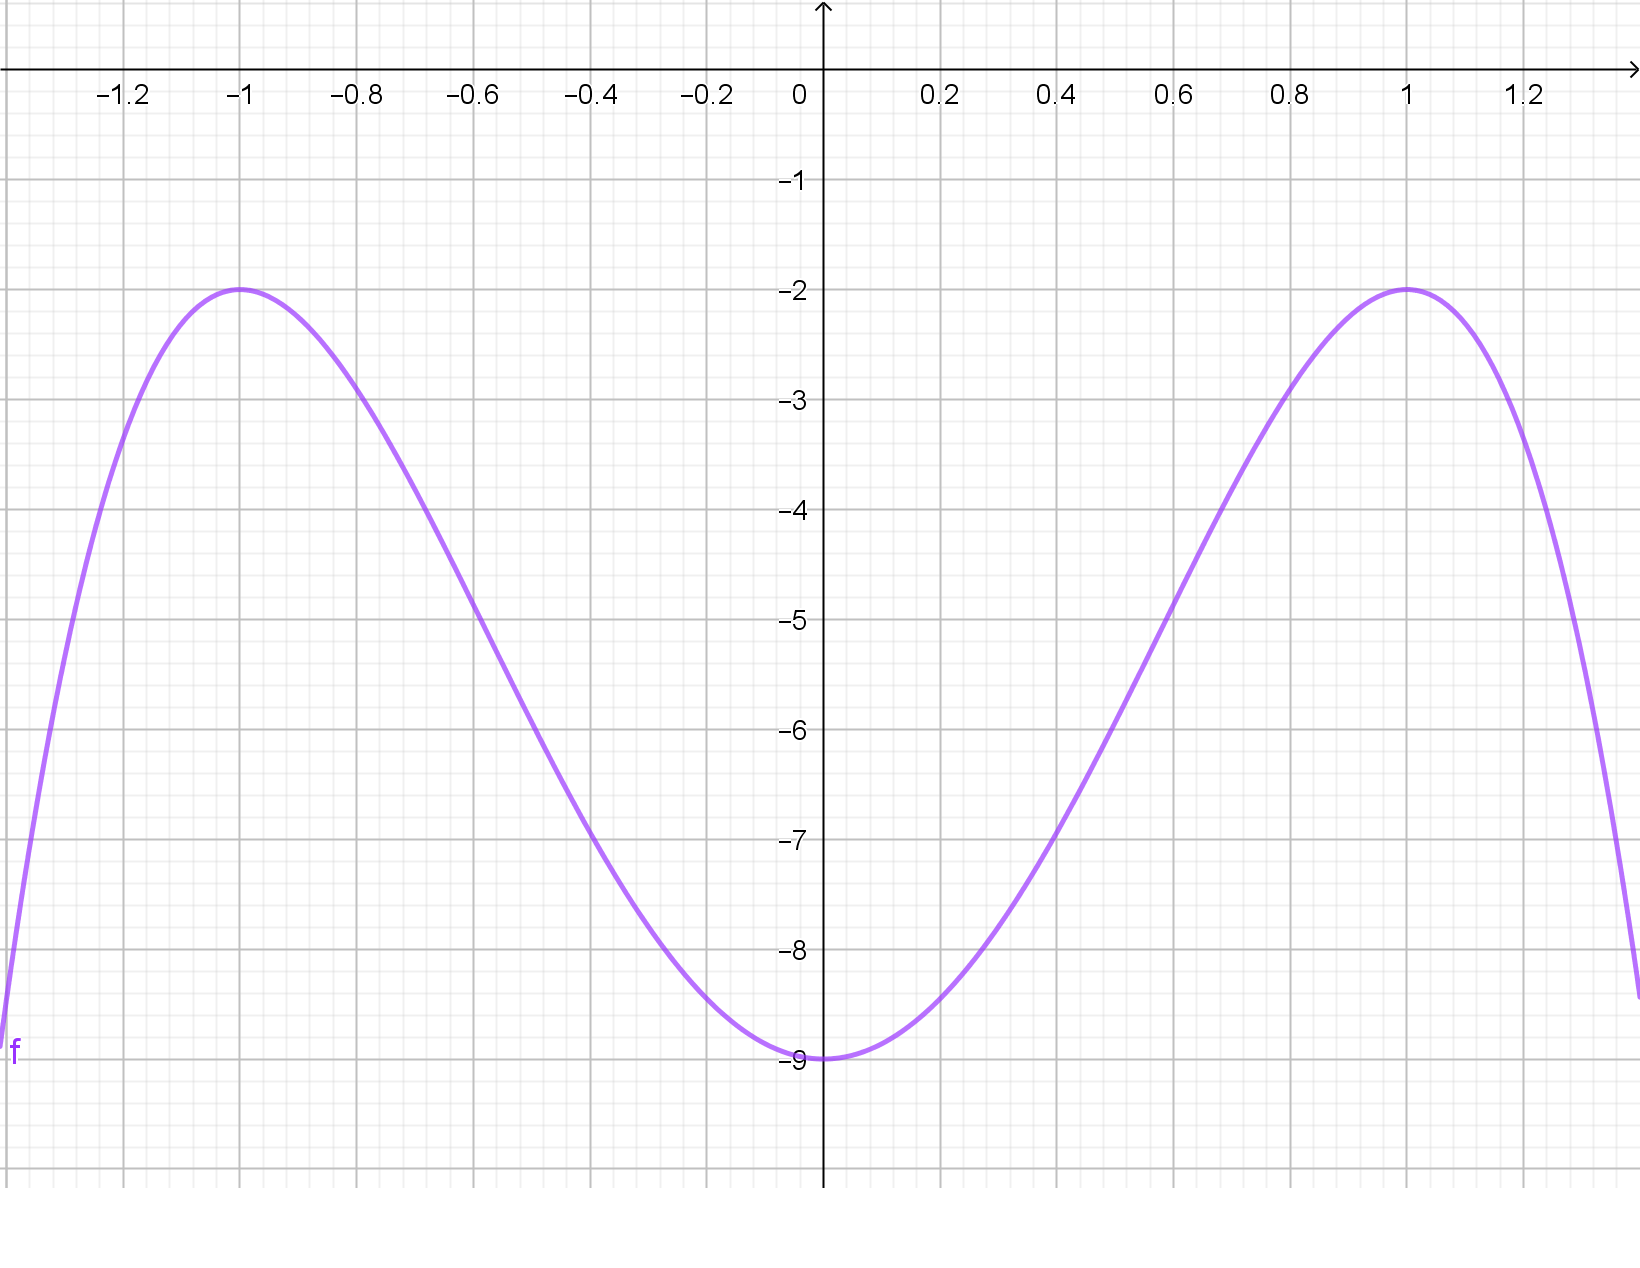
\includegraphics[scale=0.25]{Bilder/KAUebungBilder/f0.png} &
				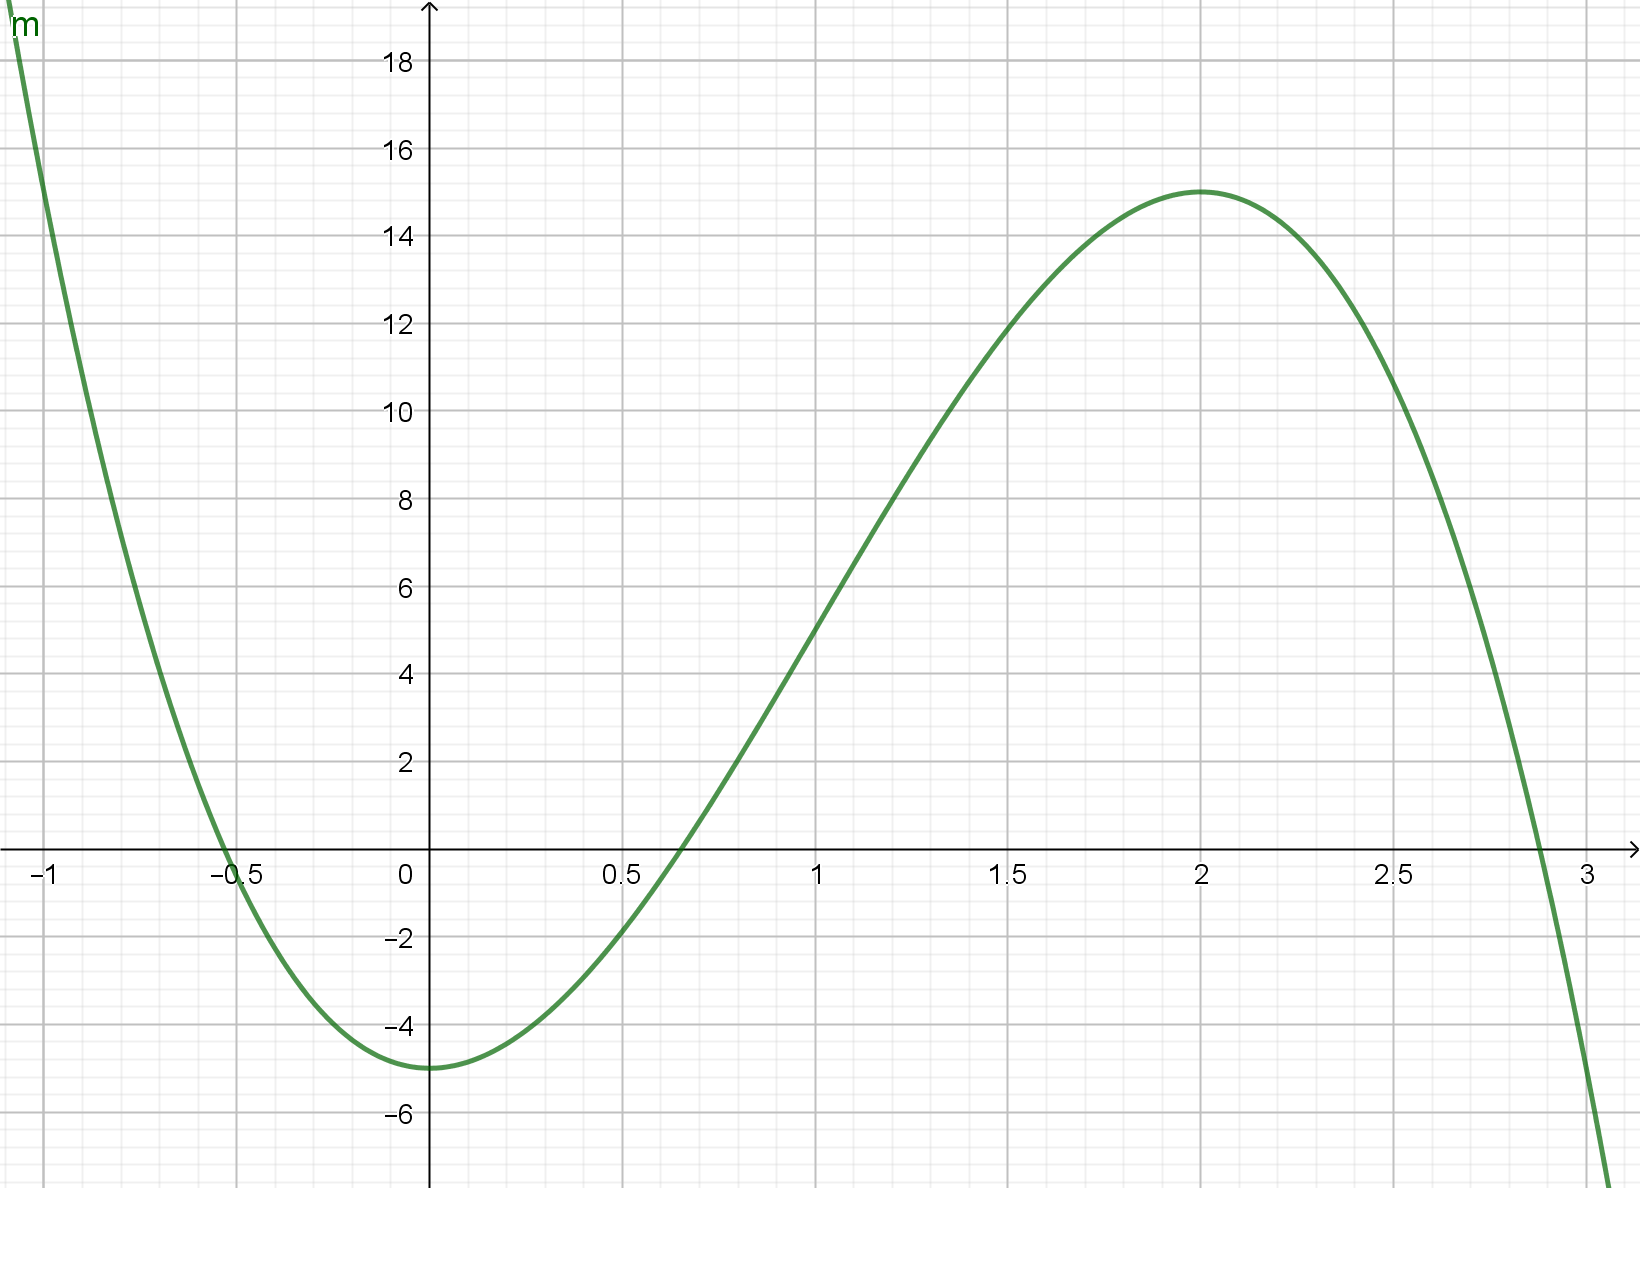
\includegraphics[scale=0.25]{Bilder/KAUebungBilder/m0.png}\\
				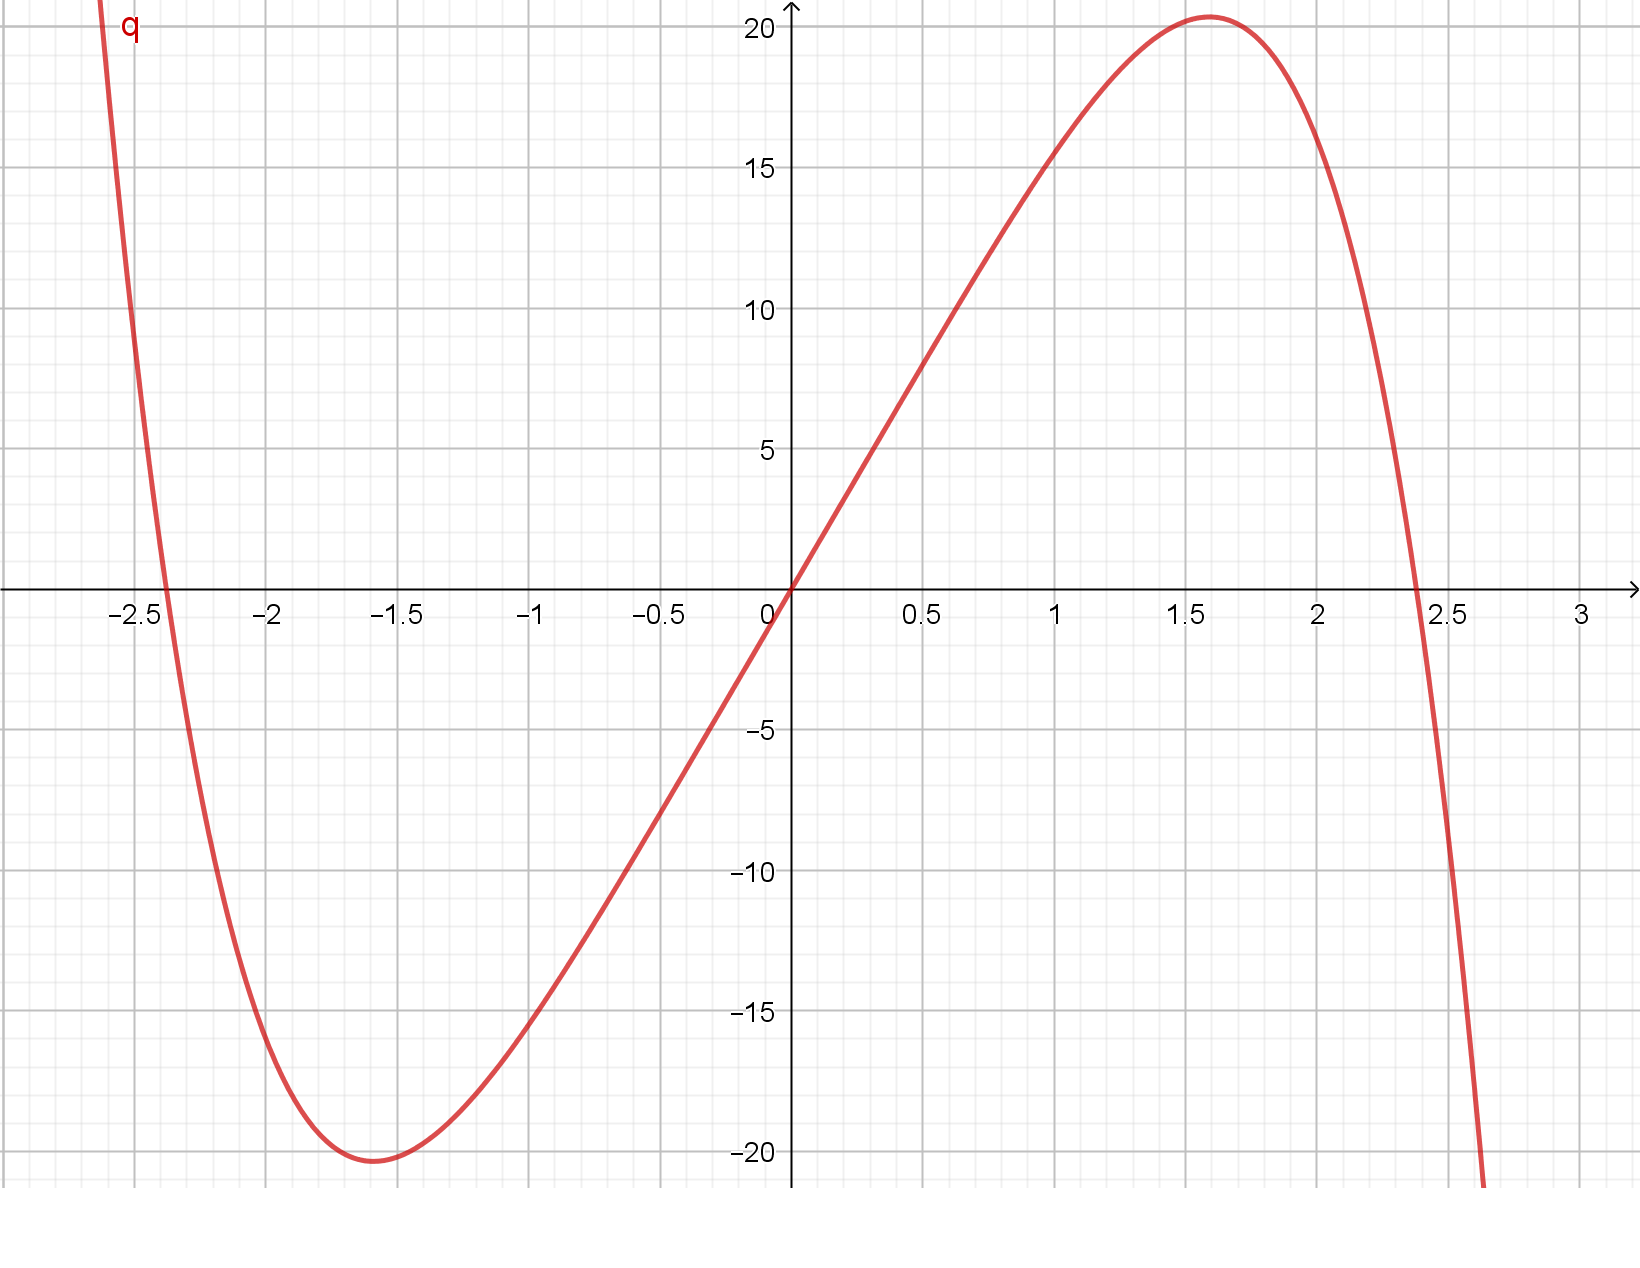
\includegraphics[scale=0.25]{Bilder/KAUebungBilder/q0.png} & 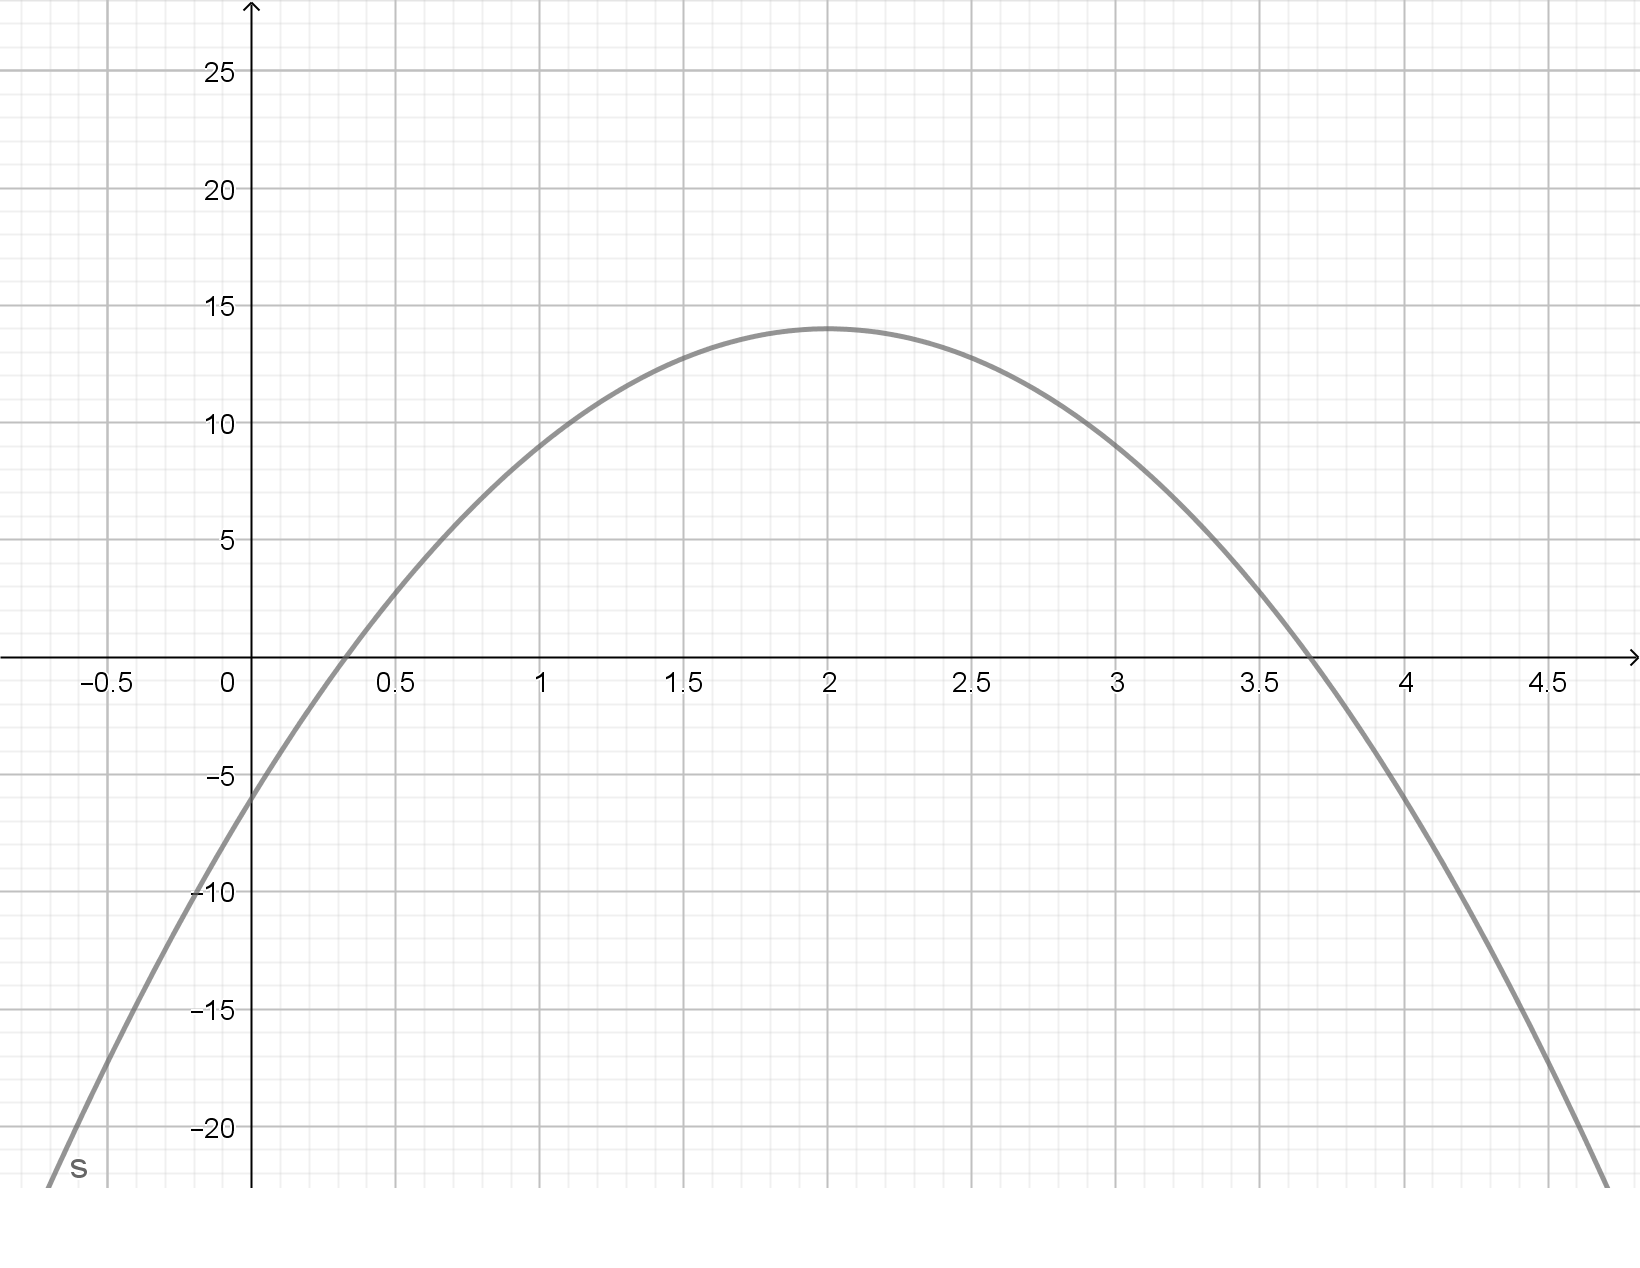
\includegraphics[scale=0.25]{Bilder/KAUebungBilder/s0.png}\\
			\end{tabularx}
			\newpage
			\noindent
			\textbf{Aufgabe 5}\\
			\indent\textbf{Aufgabe 5.1}
			Erläutern Sie, wie die ...
			\begin{itemize}
				\item[(a)] Extremstelle \(x_E\)
				\item[(b)] Wendestelle \(x_W\)
			\end{itemize}
			einer Funktion bestimmt werden kann.\\
			\hdashrule[0.2ex][x]{\textwidth}{0.2mm}{1mm 3pt}\\
			\indent\textbf{Aufgabe 5.2}\\
			Erläutern Sie, wie Sie entscheiden können, ob es sich bei \(x_E\) um einen Hoch- (HOP) oder Tiefpunkt (TIP) handelt.\\
			\hdashrule[0.2ex][x]{\textwidth}{0.2mm}{1mm 3pt}\\
			\indent\textbf{Aufgabe 5.3}\\
			Beschreiben Sie, woran Sie erkennen können, ob es sich bei \(x_W\) um...
			\begin{itemize}
				\item[(a)] einen fallenden Wendepunkt (RL)
				\item[(b)] einen steigenden Wendepunkt (LR)
			\end{itemize}
			handelt.\\
			\hdashrule[0.5ex][x]{\textwidth}{0.1mm}{8mm 2pt}\\
			\textbf{Aufgabe 6}\\
			Gegeben sind die folgenden Funktionen
			\begin{align*}
				&(a)\ f(x) = 3x^6 -18x^4+27x^2\\
				&(b)\ f(x) = -5x^3+15x^2-5\\
				&(c)\ f(x) = -\frac{1}{2}x^5 +16x\\
				&(d)\ f(x) = -5x^2+20x-6\\
				&(e)\ f(x) = 7x^4-14x^2+9\\
				&(f)\ f(x) = 10x^3-14x^2+3x
			\end{align*}
			\indent
			\textbf{Aufgabe 6.1}\\
			Berechnen Sie, wann die Funktion ein \textit{Extremwert} erreicht.\\
			Geben Sie ebenfalls das zugehörige \textit{relative Maximum} bzw. \textit{relative Minimum} an.\\
			\hdashrule[0.2ex][x]{\textwidth}{0.2mm}{1mm 3pt}\\
			\indent\textbf{Aufgabe 6.2}\\
			Bestimmen Sie, um was für eine Extremstelle es sich handelt.\\
			\hdashrule[0.2ex][x]{\textwidth}{0.2mm}{1mm 3pt}\\
			\indent\textbf{Aufgabe 6.3}\\
			Geben Sie jeweils die Stelle mit der kleinsten bzw. größten Steigung an.\\
			Bestimmen Sie den dazugehörigen Punkt.\\
			\indent\textbf{Aufgabe 6.4}\\
			Stellen Sie fest, um welche Art von Wendestelle es sich handelt.\\
			\hdashrule[0.5ex][x]{\textwidth}{0.1mm}{8mm 2pt}\\
			\textbf{Aufgabe 7}\\
			Gegeben sind die folgenden Funktionen mit den entsprechenden markanten Stellen.\\
			\begin{tabularx}{\textwidth}{lXlll}
				& Funktion & \(x_N\) & \(x_E\) & \(x_W\)\\
				\hline
				(a) & \(f(x) =  6x^2 +9\) & & \(x_{TIP}= 0\) & \\
				\hline
				(b) & \(f(x) = 2x^2-x+4\) & & \(x_{TIP} = 0,25\) & \\
				\hline
				(c) & \(f(x) = 2x^5 +3x^4-x^3-9x^2-15x\) & \(x_{N_1}=-1,73\) & \(x_{HOP} = -1,11\) & \(x_{W_{RL}}=0,6\)\\
				& & \(x_{N_2}=0\) & \(x_{TIP}=1,19\) & \\
				& & \(x_{N_3}=1,73\)& & \\
				\hline
				(d) & \(f(x) = -x^3 +x^2+8x\) & \(x_{N_1}=-2,37\) & \(x_{TIP}=-1,33\) & \(x_{W_{LR}} = 0,33\)\\
				& & \(x_{N_2} = 0\) & \(x_{HOP}=2\) & \\
				& & \(x_{N_3} = 3,37\) & & \\
				\hline
				(e) & \(f(x) = -20x^4+24x^2\) & \(x_{N_1} = -1,1\) & \(x_{HOP_1} = -0,77\) & \(x_{W_{RL}} = -0,45\)\\
				& & \(x_{N_2} = 0\) & \(x_{TIP} = 0\) & \(x_{W_{LR}= 0.45}\)\\
				& & \(x_{N_3} = 1,1\) & \(x_{HOP_2} = 0,77\) & \\
				\hline
				(f) & \(f(x) = x^3-12x-16\) & \(x_{N_1}= -2\) & \(x_{HOP} = -2\) & \(x_{W_{RL}} = 0\)\\
				& & \(x_{N_2} = 4\) & \(x_{TIP} = 2\) & \\
				\hline
				(g) & \(f(x) = x^3-4,5x^2+6,75x-3,38\) & \(x_{N_1}= 1,5\) & & \(x_{W_{RL}} = 1,5\)\\
				\hline
			\end{tabularx}\\
			\par\bigskip
			\indent
			\textbf{Aufgabe 7.1}\\
			Bestimmen Sie die Koordinaten für die Nullstellen.\\
			\hdashrule[0.2ex][x]{\textwidth}{0.2mm}{1mm 3pt}\\
			\indent\textbf{Aufgabe 7.2}\\
			Bestimmen Sie jeweils das \textit{\colorbox{blue!5}{relative Maximum}} und das \textit{\colorbox{blue!5}{relative Minimum}}.\\
			\hdashrule[0.2ex][x]{\textwidth}{0.2mm}{1mm 3pt}\\
			\indent\textbf{Aufgabe 7.3}\\
			Berechnen Sie den Punkt, an dem sich das Krümmungsverhalten des Funktionsgraphen ändert.\\
			\hdashrule[0.5ex][x]{\textwidth}{0.1mm}{8mm 2pt}\\
			\textbf{Aufgabe 8}\\
			Übertragen Sie die angegebenen Punkte in ein entsprechend skaliertes Koordinatensystem.\\
			\hdashrule[0.2ex][x]{\textwidth}{0.2mm}{1mm 3pt}\\
			\indent \textbf{(a)} Die Funktion \(f(x) = 3x^6-18x^4+27x^2\) erreicht bei \(x=-1\) und \(x=1\) den relativ gesehenen größten Wert \(y=12\). Bei \(x=-1,12\), \(x=0\) und \(x=1,12\) den relativ kleinsten Wert \(y=0\).\\
			\indent Bei \(P(-1,45|4,96)\) und \(Q(0,53|6,28)\) wechselt der Graph von einer \textit{Linkskrümmung} zu einer \textit{Rechtskrümmung}. Im gegensatz ändert sich die Krümmung von \textit{rechts} zu \textit{links} bei \(R(-0,53|6,28)\) und \(S(1,45|4,96)\).\\
			\hdashrule[0.2ex][x]{\textwidth}{0.2mm}{1mm 3pt}\\
			\indent \textbf{(b)} Das Krümmungsverhalten der Funktion \(f(x) = -5x^3 +15x^2-5\) wechselt für \(W(1|5)\) von \textit{linksgekrümmt} zu \textit{rechtsgekrümmt}.\\
			Ein \textit{relatives Maximum} hat \(f(x)\) bei \(H(2|15)\). Das \textit{relative Minimum} hingegen liegt in \(T(0|-5)\).\\
			\hdashrule[0.2ex][x]{\textwidth}{0.2mm}{1mm 3pt}\\
			\indent \textbf{(c)}
		\end{framed}
	\end{worksheet}
\end{document}